\documentclass[10pt]{article}
\usepackage[ngerman]{babel}
\usepackage[utf8]{inputenc}
\usepackage[T1]{fontenc}
\usepackage{amsmath}
\usepackage{amsfonts}
\usepackage{amssymb}
\usepackage[version=4]{mhchem}
\usepackage{stmaryrd}
\usepackage{graphicx}
\usepackage[export]{adjustbox}
\graphicspath{ {./images/} }

\title{Hauptprüfung Abiturprüfung 2021 - Leistungsfach }

\author{Alexander Schwarz\\
www.mathe-aufgaben.com}
\date{}


\begin{document}
\maketitle
 Baden-WürttembergAugust 2021

\section*{Aufgabe A 2.1}
Die Funktion f beschreibt für $0 \leq \mathrm{t} \leq 8$ modellhaft die Wachstumsgeschwindigkeit eines Apfelbaums, der zu Beobachtungsbeginn 0,8m hoch ist (t in Jahren nach Beobachtungsbeginn, $f(t)$ in Meter pro Jahr).\\
a) Die Abbildung in der Anlage zeigt den Graphen $G_{f}$ von $f$.

Bestimmen Sie die Länge des Zeitraums, in dem die Wachstumsgeschwindigkeit des Apfelbaums größer als 0,5 Meter pro Jahr ist.\\
(1 VP)\\
Bestimmen Sie die Höhe des Apfelbaums zwei Jahre nach Beobachtungsbeginn.\\
(2 VP)\\
Die Wachstumsgeschwindigkeit eines Birnbaums, der zu Beobachtungsbeginn 1,2 m hoch ist, wird für $0 \leq t \leq 8$ modellhaft beschrieben durch die Funktion g mit $\mathrm{g}(\mathrm{t})=\mathrm{t}^{2} \cdot \mathrm{e}^{-\mathrm{t}}$ (t in Jahren nach Beobachtungsbeginn, $\mathrm{g}(\mathrm{t})$ in Meter pro Jahr).

Für die Ableitungen der Funktion g gilt:\\
$g^{\prime}(t)=2 t \cdot e^{-t}-t^{2} \cdot e^{-t} \quad g^{\prime \prime}(t)=2 e^{-t}-4 t \cdot e^{-t}+t^{2} \cdot e^{-t}$\\
b) Berechnen Sie den Zeitpunkt, zu dem die Wachstumsgeschwindigkeit des Birnbaums am größten ist, und geben Sie diese Wachstumsgeschwindigkeit an.\\
(2 VP)\\
Begründen Sie, dass der Birnbaum ab diesem Zeitpunkt weiterhin wächst, die Wachstumsgeschwindigkeit jedoch ständig abnimmt.\\
(2 VP)\\
Formulieren Sie eine Frage im Sachzusammenhang, die auf die Gleichung\\
$\frac{1}{5} \cdot \int_{x}^{x+5} g(t) d t=0,3$ führt.\\
c) Zeigen Sie, dass für $0 \leq t \leq 8$ die Funktion h mit\\
$h(t)=\left(-t^{2}-2 t-2\right) \cdot e^{-t}+3,2$\\
die Höhe des Birnbaums beschreibt ( t in Jahren nach Beobachtungsbeginn, $\mathrm{h}(\mathrm{t})$ in Meter).\\
(2 VP)\\
d) Durch die Zugabe eines Düngers wird das Wachstums von Birnbäumen beeinflusst. Die Höhe eines gedüngten Birnbaums wird durch die Funktion k beschrieben mit $k(t)=-2,3 e^{-t}+3,5$\\
( $t \geq 0$ in Jahren nach Beobachtungsbeginn, $k(t)$ in Meter).\\
Die Höhe eines ungedüngten Birnbaums wird weiterhin durch die Funktion h beschrieben. Beide Birnbäume haben zu Beobachtungsbeginn dieselbe Höhe. Berechnen Sie den Zeitpunkt, bis zu dem die Wachstumsgeschwindigkeit des gedüngten Birnbaums größer ist als die des ungedüngten Birnbaums. Untersuchen Sie rechnerisch, welcher der beiden Bäume zuerst eine Höhe von $3,1 \mathrm{~m}$ erreicht.

\section*{Aufgabe A 2.2}
Für jedes $t>0$ ist eine Funktion $f_{t}$ gegeben durch $f_{t}(x)=-4 x^{3}+12 t x^{2}$.\\
a) Bestimmen Sie die Nullstellen von $f_{t}$.

Der Graph von $f_{t}$ schließt mit der x-Achse eine Fläche mit dem Inhalt $A_{t}$ ein. Ermitteln Sie denjenigen Wert von $t$, für den $A_{t}=\frac{16}{3}$ gilt.\\
b) Für $t=\frac{2}{3}$ gibt es Tangenten an den Graphen von $f_{t}$, die den Punkt $S(3 \mid 0)$ enthalten.\\
Berechnen Sie die x-Koordinaten der zugehörigen Berührpunkte.

\section*{Abbildung zu Aufgabe A 2.1}
\begin{center}
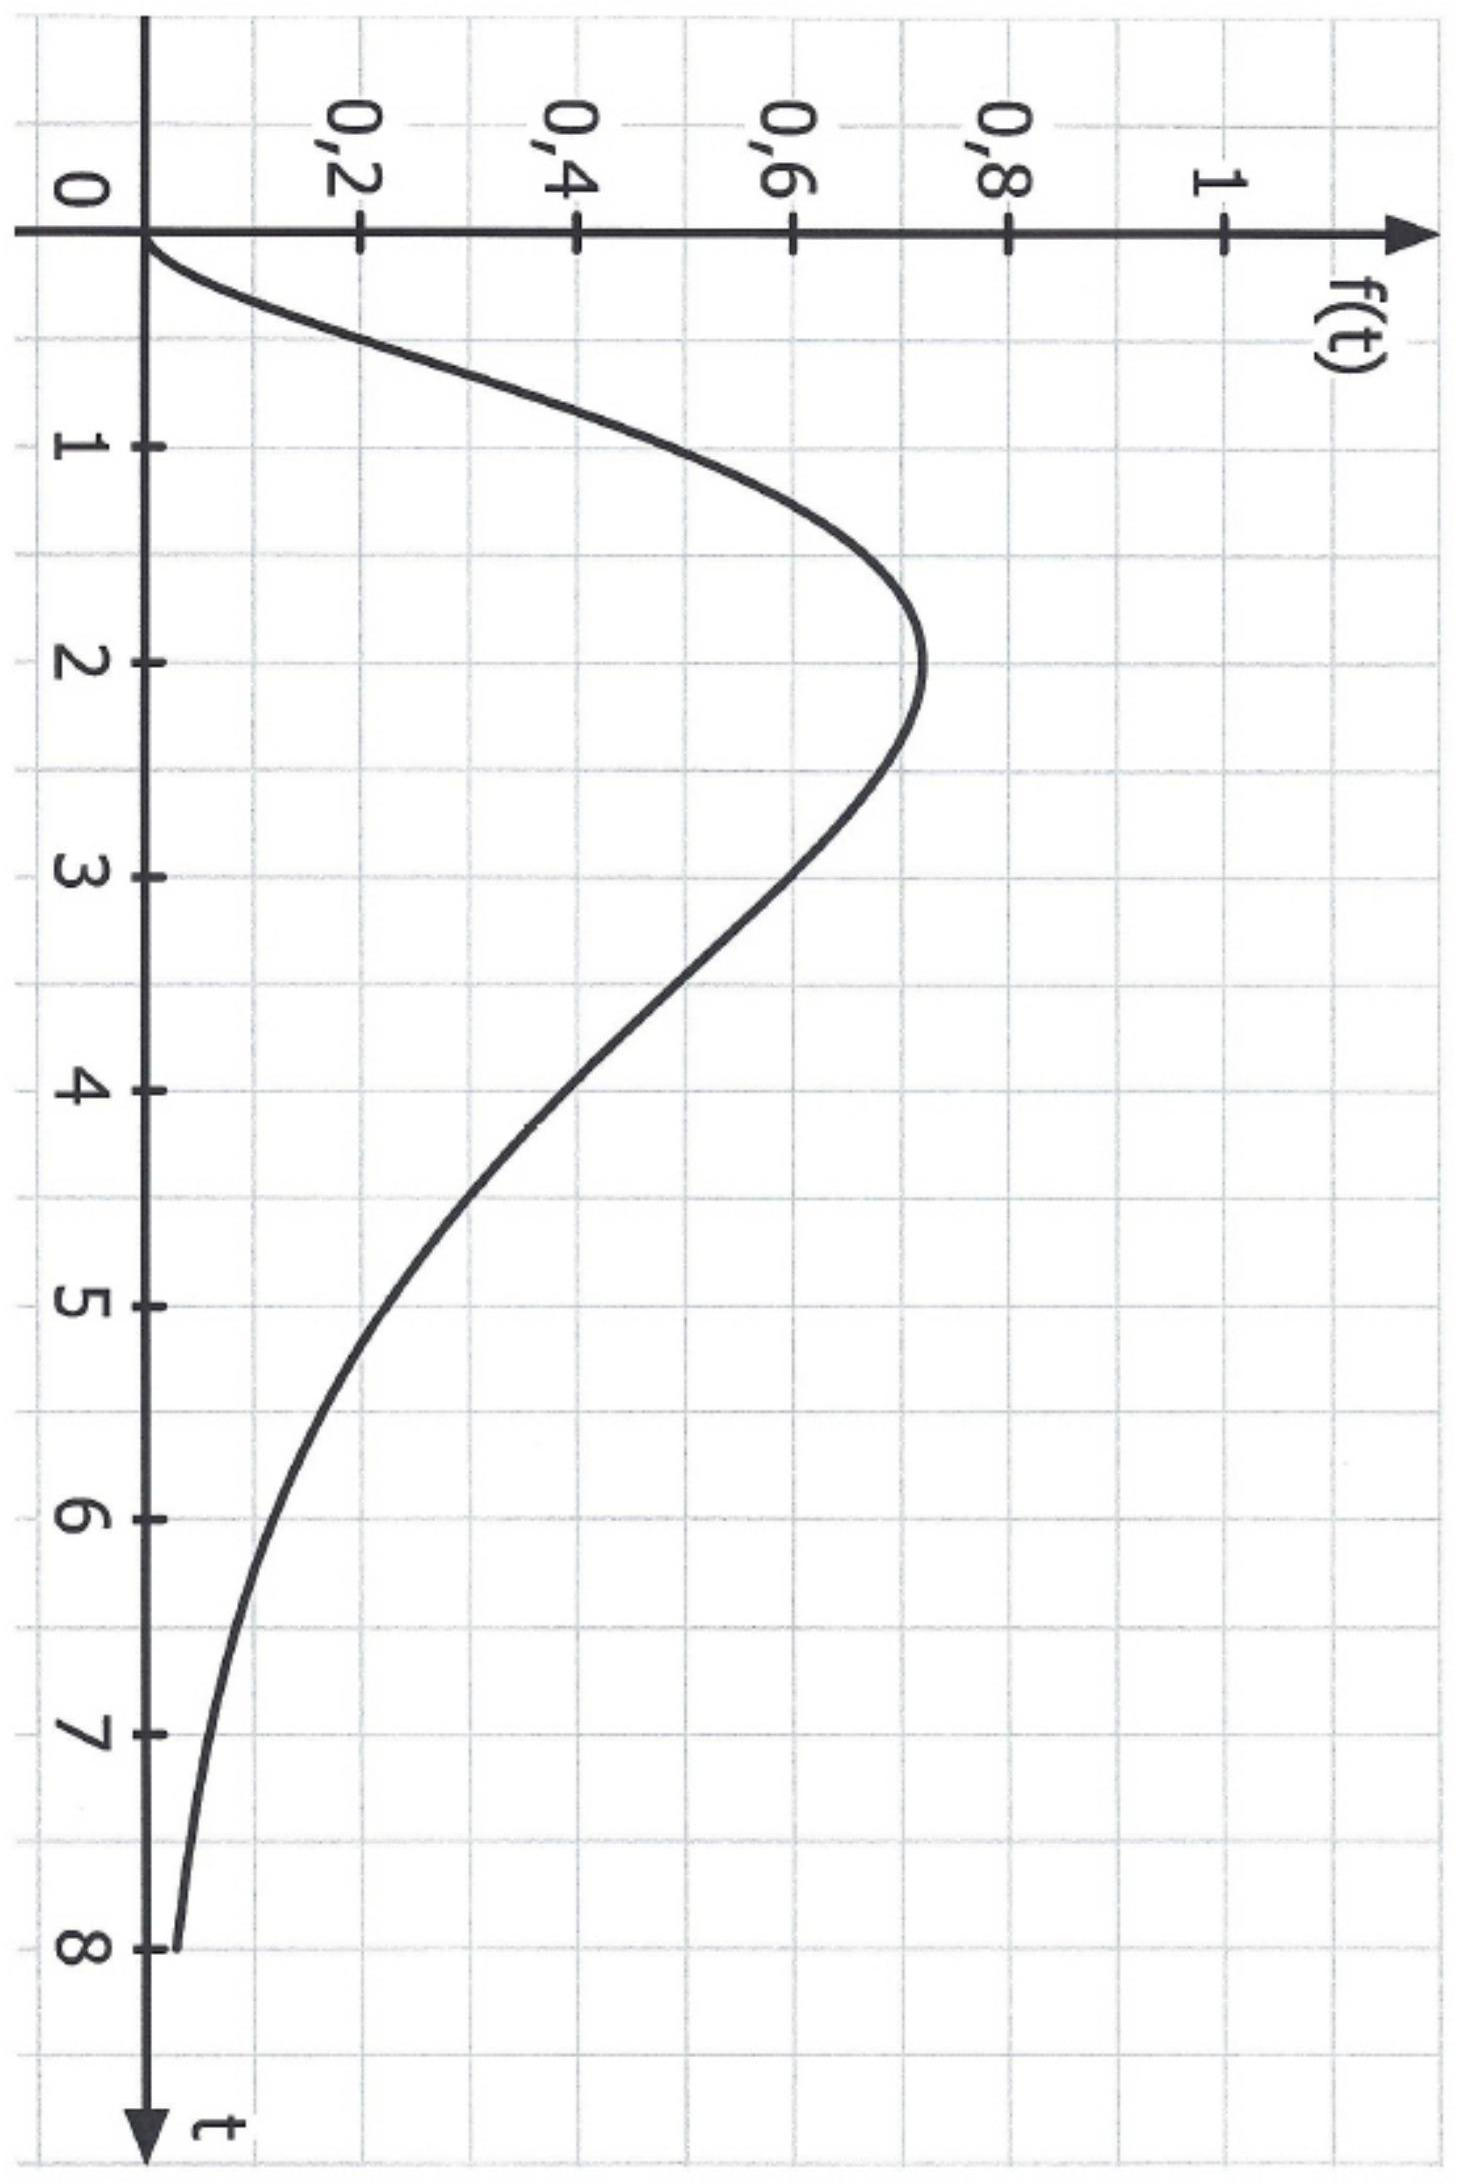
\includegraphics[max width=\textwidth]{2025_04_24_88bfd1c98384e043e4f6g-4}
\end{center}

\section*{Lösungen}
\section*{Aufgabe A 2.1}
a) Bestimmen Sie die Länge des Zeitraums, in dem die Wachstumsgeschwindigkeit des Apfelbaums größer als 0,5 Meter pro Jahr ist.

Aus dem Schaubild von $f$ kann man ablesen.\\
$f(1) \approx 0,5$ und $f(3,5) \approx 0,5$\\
Der gesuchte Zeitraum beträgt ca. 2,5 Jahre.

Bestimmen Sie die Höhe des Apfelbaums zwei Jahre nach Beobachtungsbeginn.\\
Die Höhe des Apfelbaums berechnet sich mit der Formel $0,8+\int_{0}^{2} f(t) d t$.\\
Das Integral kann man anschaulich mit Hilfe des Schaubilds von f näherungsweise bestimmen.\\
1 Kästchen entspricht einer Höhe von 0,5Jahre $\cdot 0,1 \frac{\mathrm{Meter}}{\mathrm{Jahr}}=0,05$ Meter\\[0pt]
Im Intervall [0;2] befinden sich zwischen dem Schaubild von f und der t-Achse ungefähr 17 Kästchen.

Daraus folgt $0,8+\int_{0}^{2} f(t) d t \approx 0,8+17 \cdot 0,05=1,65$ Meter\\
Nach 2 Jahren ist der Baum ungefähr 1,65 Meter hoch.\\
b) Berechnen Sie den Zeitpunkt, zu dem die Wachstumsgeschwindigkeit des

Birnbaums am größten ist, und geben Sie diese Wachstumsgeschwindigkeit an.\\
Gesucht ist die Stelle, an der sich der Hochpunkt des Schaubildes von g befindet.\\
Hinreichende Bedingung für den Hochpunkt: $\mathrm{g}^{\prime}(\mathrm{t})=0$ und $\mathrm{g}^{\prime \prime}(\mathrm{t})<0$\\
$2 t \cdot e^{-t}-t^{2} \cdot e^{-t}=0$\\
$\Leftrightarrow t \cdot e^{-t} \cdot(2-t)=0$\\
Lösung mit dem Satz vom Nullprodukt ergibt $\mathrm{t}=0$ oder $\mathrm{t}=2$\\
$\mathrm{g}^{\prime \prime}(0)=2>0$; bei $\mathrm{t}=0$ liegt ein Tiefpunkt vor\\
$\mathrm{g}^{\prime \prime}(2)=2 \mathrm{e}^{-2}-8 \mathrm{e}^{-2}+4 \mathrm{e}^{-2}=-2 \mathrm{e}^{-2}<0$\\
Somit ist die Wachstumsgeschwindigkeit nach 2 Jahren maximal.\\
Die maximale Geschwindigkeit beträgt $g(2)=4 \mathrm{e}^{-2} \approx 0,54$ Meter pro Jahr

Begründen Sie, dass der Birnbaum ab diesem Zeitpunkt weiterhin wächst, die Wachstumsgeschwindigkeit jedoch ständig abnimmt.

Für $\mathrm{t}>2$ ist $\mathrm{g}(\mathrm{t})>0$.\\
Das heißt, dass die Wachstumsgeschwindigkeit auch für t>2 positiv ist und der Baum auch nach 2 Jahren weiterhin wächst.

Für $\mathrm{t}>2$ ist $\mathrm{g}^{\prime}(\mathrm{t})=\mathrm{t} \cdot \mathrm{e}^{-\mathrm{t}} \cdot(2-\mathrm{t})<0$, da $\mathrm{t} \cdot \mathrm{e}^{-\mathrm{t}}>0$ und $2-\mathrm{t}<0$ ist.\\
Damit ist die Funktion g für $\mathrm{t}>2$ streng monoton fallend.\\
Das heißt, dass die Wachstumsgeschwindigkeit für $\mathrm{t}>2$ abnimmt.

Formulieren Sie eine Frage im Sachzusammenhang, die auf die Gleichung $\frac{1}{5} \cdot \int_{x}^{x+5} g(t) d t=0,3$ führt.

Bei der Integralformel handelt es sich um die Mittelwertformel.\\
Gesucht ist der Beginn eines 5-Jahresintervall [ $x$; $x+5$ ], in welchem die mittlere Wachstumsgeschwindigkeit 0,3 Meter pro Jahr beträgt.\\
c) Es ist zu zeigen, dass die Funktion $h$ eine Stammfunktion von $g$ ist.\\
$h^{\prime}(\mathrm{t})=(-2 \mathrm{t}-2) \cdot \mathrm{e}^{-\mathrm{t}}+\left(-\mathrm{t}^{2}-2 \mathrm{t}-2\right) \cdot \mathrm{e}^{-\mathrm{t}} \cdot(-1)=\mathrm{e}^{-\mathrm{t}}\left(-2 \mathrm{t}-2+\mathrm{t}^{2}+2 \mathrm{t}+2\right)=\mathrm{t}^{2} \cdot \mathrm{e}^{-\mathrm{t}}$\\
Somit ist $\mathrm{h}^{\prime}(\mathrm{t})=\mathrm{g}(\mathrm{t})$, also ist die Stammfunktionseigenschaft bestätigt.\\
Weiterhin gilt auch $h(0)=1,2$ was der Anfangshöhe des Baumes entspricht.\\
d) Berechnen Sie den Zeitpunkt, bis zu dem die Wachstumsgeschwindigkeit des gedüngten Birnbaums größer ist als die des ungedüngten Birnbaums.

Gesucht ist der Zeitpunkt $t$, für den gilt: $k^{\prime}(t)>g(t)$\\
Es gilt $k^{\prime}(t)=2,3 e^{-t}$\\
$2,3 e^{-t}>t^{2} \cdot e^{-t} \quad \mid: e^{-t} \quad$ (Division ist erlaubt, da $e^{-t} \neq 0$ ist)\\
$\Leftrightarrow t^{2}<2,3$\\
$\Rightarrow-\sqrt{2,3}<\mathrm{t}<\sqrt{2,3} \approx 1,52$\\
Bis etwa 1,5 Jahre nach Beobachtungsbeginn wächst der gedüngte Baum schneller als der ungedüngte Baum.

Untersuchen Sie rechnerisch, welcher der beiden Bäume zuerst eine Höhe von 3,1 m erreicht.

Zeitpunkt, zu dem der gedüngte Baum 3,1m hoch ist: $k(t)=3,1$\\
$-2,3 \mathrm{e}^{-\mathrm{t}}+3,5=3,1 \quad \Leftrightarrow \mathrm{e}^{-\mathrm{t}}=\frac{0,4}{2,3} \Leftrightarrow \mathrm{t}=-\ln \left(\frac{0,4}{2,3}\right) \approx 1,75$\\
Der gedüngte Baum ist nach 1,75 Jahren 3,1 Meter hoch.\\
Höhe des ungedüngten Baumes nach 1,75 Jahren: $h(1,75) \approx 1,71<3,1$ Meter\\
Somit erreicht der gedüngte Baum zuerst eine Höhe von 3,1 Meter.

\section*{Aufgabe A 2.2}
a) Bestimmen Sie die Nullstellen von $f_{t}$.

$$
f_{t}(x)=0:-4 x^{3}+12 t x^{2}=0 \quad \Leftrightarrow x^{2} \cdot(-4 x+12 t)=0
$$

Lösung mit dem Satz vom Nullprodukt: $x_{1}=0$ und $x_{2}=3 t$\\
Ermitteln Sie denjenigen Wert von $t$, für den $\mathrm{A}_{\mathrm{t}}=\frac{16}{3}$ gilt.\\
$\int_{0}^{3 t} f_{t}(x) d x=\left[-x^{4}+4 t x^{3}\right]_{0}^{3 t}=-(3 t)^{4}+4 t \cdot(3 t)^{3}=-81 t^{4}+108 t^{4}=27 t^{4}$\\
Bedingung: $27 t^{4}=\frac{16}{3} \Leftrightarrow t= \pm \sqrt[4]{\frac{16}{81}}= \pm \frac{2}{3}$\\
Da $\mathrm{t}>0$ ist, kommt nur $\mathrm{t}=\frac{2}{3}$ in Betracht.\\
b) Es gilt $\mathrm{f}_{\frac{2}{3}}(\mathrm{x})=-4 \mathrm{x}^{3}+8 \mathrm{x}^{2}$ und $\mathrm{f}_{\frac{2}{3}}^{\prime}(\mathrm{x})=-12 \mathrm{x}^{2}+16 \mathrm{x}$

Vom Punkt $\mathrm{S}(3 \mid 0)$ aus werden Tangenten an das Schaubild von g angelegt.\\
Allgemeine Tangentengleichung: $y=f_{\frac{2}{3}}^{\prime}(u) \cdot(x-u)+f_{\frac{2}{3}}(u)$\\
Einsetzen des Punktes $\mathrm{S}(3 \mid 0)$ :\\
$0=\left(-12 u^{2}+16 u\right) \cdot(3-u)-4 u^{3}+8 u^{2}$\\
$\Leftrightarrow 0=-36 u^{2}+12 u^{3}+48 u-16 u^{2}-4 u^{3}+8 u^{2}$\\
$\Leftrightarrow 0=8 u^{3}-44 u^{2}+48 u$\\
$\Leftrightarrow u \cdot\left(8 u^{2}-44 u+48\right)=0 \quad$ Lösung mit dem Satz vom Nullprodukt\\
I) $u_{1}=0$\\
II) $8 u^{2}-44 u+48=0 \quad$ abc-Formel: $u_{2,3}=\frac{44 \pm 20}{16} \quad u_{2}=4 \quad u_{3}=1,5$

Die x-Koordinaten der Berührpunkte sind 0, 1,5 und 4 .


\end{document}